%!TEX root = ../thesis.tex
\section{Automatic Effect Decision Pipeline}
DemoCut performs several automated steps to convert the user-annotated
input recording into an edited video tutorial. First, the system segments the recording into regions around user-specified markers. This segmentation considers both the
similarity of video frames around each marker and the presence of
narration in the audio track in order to determine the appropriate
segment boundaries (Figure~\ref{fig:democut_pipeline}). DemoCut then automatically applies an temporal and a visual effect to
each segment based on the type of the corresponding user marker and
the properties of the audio/video content in the segment. The rest of
this section describes these steps in detail.

\begin{figure}[b]
  \centering
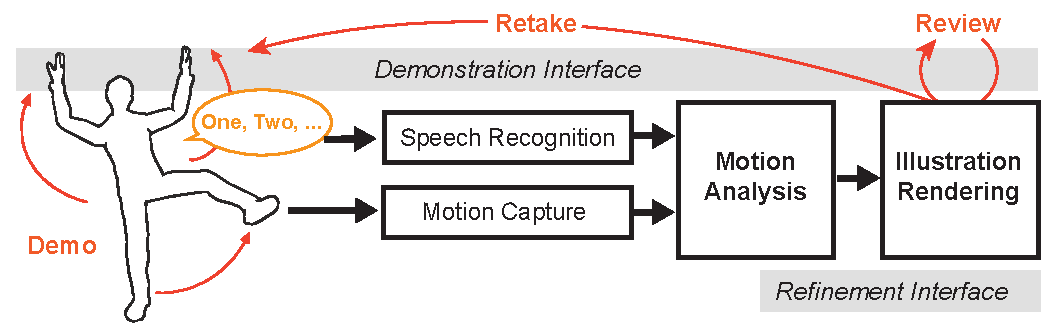
\includegraphics[width=0.8\columnwidth]{\democut/fig/pipeline}
  \caption{Given user markers, DemoCut analyzes both video and audio to segment the demonstration video and apply editing effects.}
  \label{fig:democut_pipeline}
\end{figure}

\begin{figure}[t]
  \centering
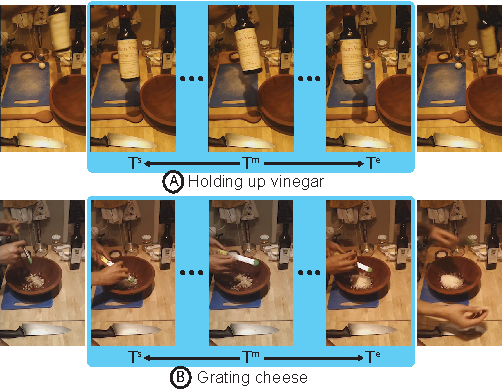
\includegraphics[width=0.6\columnwidth]{\democut/fig/video-similarity}
  \caption{DemoCut looks for similar video frames before and
after a marked frame $T^m$ to find candidate start ($T^s$) and end ($T^e$) frames
for the corresponding segment.}
 \label{fig:video-similarity}
\end{figure}

\subsection{Video Segmentation}

Except for the step marker, all of the user-specified markers indicate
important moments in the demonstration that correspond to some segment
of the recording. In many cases, we can infer the duration of these
segments by searching for video frames that look similar to the marked
frame. For example, in Figure~\ref{fig:video-similarity}A, the similar
frames before and after a supply marker show the author holding up a
bottle of vinegar, and in Figure~\ref{fig:video-similarity}B, the
similar frames around an action marker show the author grating cheese.
%
For every marked frame $T^m$, DemoCut uses the following method to
compute candidate start and end frames $T^s$ and $T^e$ for the
corresponding segment.
%
For the $i$-th marked frame $T_i^m$, our algorithm finds $T_i^s$ by
comparing $T_i^m$ to earlier frames in the video until it reaches a
previous marker at $T_{i-1}^m$, or until 5\% of pixels (in grayscale)
%in the grayscale versions of the frames
have changed by 20\%. Similarly, the system
finds $T_i^e$ by comparing $T_i^m$ to subsequent frames in the video.
To optimize performance, DemoCut compares to frames sampled at 0.5
seconds and ignores overlaps between segments. Segment overlaps are
resolved during boundary adjustment after incorporating the audio
analysis.

\subsection{Adjusting Segments with Audio Analysis}

Adjacent segments can have different effects that change how video and audio are processed. To prevent such changes from interfering with a video's narration, DemoCut adjusts segment boundaries to align with audio activity boundaries.
% DemoCut chooses different editing effects for different
% segments. Segment boundaries should therefore be carefully adjusted based on the audio
% track to avoid interrupting the author's narration.

\begin{figure}[t]
  \centering
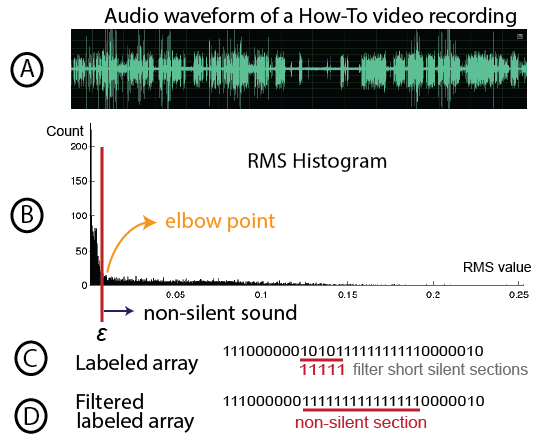
\includegraphics[width=0.8\columnwidth]{\democut/fig/audio}
  \caption{We use RMS energy of the audio to find silent and non-silent regions. We determine the threshold for silence by analyzing the histogram of the RMS energy.}
  \label{fig:audio}
\end{figure}

\subsubsection{Detecting non-silent sections}
%
Since many DIY videos include prominent non-speech sounds such as
chopping noises, power tools, etc., detecting speech automatically is
a challenging task. We found that even state-of-the-art speech
detection algorithms produce poor results in many cases.
%
As a result, we take a more conservative approach; DemoCut
automatically detects non-silent sections in the recorded
audio and treats the background sound as part of the narration.

At a high level, our algorithm for detecting non-silent sections works
as follows. We compute the ``loudness'' of each audio window,
organize the windows into a histogram based on loudness, and then
analyze the histogram to determine a minimum loudness threshold for
non-silent windows. We then apply this threshold to categorize all
audio windows as silent or non-silent. Finally, we filter this
categorization to eliminate very short sequences of silent or non-silent samples. Here, we describe these steps in more detail:
% \bh{I think we mean "window" instead of "sample" for the preceding section, since RMS operates on windows.}

\emph{Computing loudness.} Given an input audio waveform sampled at
44.1 kHz (Figure~\ref{fig:audio}A), we estimate loudness by computing
the root mean square (RMS) energy~\cite{Panagiotakis:2005eb} across
the entire waveform. The RMS energy
for a window of size $n$ is $\sqrt{(\sum_{n}{x_i^2})/n}$ where $x_i$ is the value of
the $i$th audio sample in the window. We set window sizes as 0.1 second with $n = 4410$. Prior to computing RMS energy, the audio is normalized and noise-reduced with Adobe Audition.

\emph{Computing loudness threshold.} After analyzing the RMS energy
profiles of several different types of DIY videos, we found that the
vast majority of recorded audio represents background sound, which
tends to have similar and fairly low RMS energy values. In contrast,
user narration varies from medium to high RMS values based on the
speaker's distance to the microphone and the sensitivity of the
recording device. Based on this observation, we first compute a histogram
of RMS energy for all windows in the audio track; the windows that
correspond to background sound form a large mass at the low-RMS end of
the histogram (Figure~\ref{fig:audio}B).
%
To distinguish these ``silent'' parts of the recording from the
narration, we smooth the histogram with a Gaussian kernel, find the
minimum derivative point in the smoothed histogram, and set the
loudness threshold $\varepsilon$ to be the RMS energy value at this
elbow point.
%
Figure~\ref{fig:audio}B shows the RMS histogram and loudness threshold
for one of our example videos, ``How to make salad dressing.''

\emph{Categorizing silent/non-silent sections.} To partition the audio
track into silent and non-silent sections, we first label each window
as silent or non-silent based on $\varepsilon$.
%
This initial labeling often includes some very short silent and
non-silent sections.
%
Since many short silent sections correspond to short pauses between
spoken words, we turn any silent sections that are shorter than 0.4
seconds into non-silent sections.
%
Then, we discard any non-silent sections that are shorter than 0.8
seconds to account for any clicks and pops in the recorded audio.
%
The 0.4 and 0.8 second thresholds for silent and non-silent sections
were tuned experimentally, and we used these parameter values for all
of our results.

\subsubsection{Adjusting segment boundaries}

In order to avoid cutting off an author's narration, DemoCut
adjusts the video segment boundaries using the non-silent sections
of the audio track (Figure~\ref{fig:democut_pipeline}). First, for any segment
%[$T_i^s$, $T_i^e$]
we find
all of the overlapping non-silent audio sections and then grow the
segment so that it completely contains all of these non-silent sections.
%
Next, DemoCut resolves overlapping segments: If any two segments
overlap,
%such that $T_{i}^{e} > T_{i+1}^{s}$,
the boundaries must be readjusted.
%
If the overlap region is silent, the region is split into two equal parts and each is assigned to the
corresponding segment.
%
If the overlap region includes a non-silent audio section,
DemoCut assigns this non-silent section to the segment that has
more overlap with the section. If the overlap for both video segments is the same, DemoCut assigns the section to the smaller video segment.
%
Finally, DemoCut addresses any gaps between segments. If a gap is less
than 2 seconds, it is merged to the shorter adjacent segment.
Otherwise, DemoCut creates a new segment for the gap. Note
that such {\em unmarked segments} do not have a corresponding marker, but
they may still show useful details of the demonstration.


%Using the non-silent sections of the audio track, DemoCut adjusts the video segment boundaries for each user-specified marker (Figure \ref{fig:audio}C). For a marker at $T_i^m$ with a shot boundary [$T_i^s$, $T_i^e$] where  $T_{i}^{s} > T_{i-1}^{e}$ and $ T_{i}^{e} < T_{i+1}^{s}$, we find all the overlapped non-silent sections during this time interval: {[$S_j^s$, $S_j^e$], [$S_{j+1}^s$, $S_{j+1}^e$], \ldots, [$S_{j+k}^s$, $S_{j+k}^e$]}.
%
%In order to have each video segment contains complete narration without a sound cutoff, we examine the first and last non-silent section and adjust the segment boundary to [$ min(T_{i}^{s}, S_{j}^{s}), max(T_{i}^{e}, S_{j+k}^{e}) $].
% Note: avoid sound cutoff if a segment is "skipped"

%After all the annotated segments are adjusted, for any two consecutive segments where their boundaries are overlapped that $T_{i}^{e} > T_{i+1}^{s}$ by $x$ seconds, if they share one speech section [$S_j^s$, $S_j^e$], assign this speech section to the video segment that overlaps more and adjust the start and end frames, i.e. either $T_{i}^{e'} = S_{j}^{e}$ or $T_{i+1}^{s'} = S_{j}^{s}$ so that $T_{i}^{e'} < T_{i+1}^{s'}$. If there is no speech section in the overlapped time frame, split into half, i.e. $T_{i}^{e'} = T_{i}^{e} + x/2$ and $T_{i+1}^{s'} = T_{i+1}^{s} - x/2$ (Figure \ref{fig:audio}D).

%In order to completely segment the entire recording, for any gap between annotated segments, if it falls below 2 seconds, merge to the shorter adjacent segment; otherwise, create an empty segment (Figure \ref{fig:audio}E).

\subsection{Applying Effects}

To automatically apply an effect to each
computed segment, DemoCut first detects whether
there is motion in the video. A segment is considered to be {\em static}
(i.e., no motion) if less than 1\% of pixels in the grayscale versions
of consecutive frames have changed by more than 20\%. To optimize for
performance, the segment is sampled at 0.5 seconds for this
comparison.
%
DemoCut chooses effects as follows:

\begin{enumerate}
  \item If the segment includes a \emph{cutout} marker, apply {\em ``Skip''}.
  \item If the segment includes a \emph{closeup} marker, apply {\em ``Zoom''} to the entire segment.
  \item If the segment includes any non-silent audio sections, apply {\em ``Fast Motion''}.
  \item If the segment is silent, static, and unmarked, apply {\em ``Skip''}.
  \item If the segment is silent but not static (either marked or unmarked), apply {\em ``Normal''}.
  \item For any marker with a text annotation, apply {\em ``Subtitles''}.

  \end{enumerate}
% \bh{Missing discussion of how to apply zoom and subtitles here. I think zoom is applied to the whole shot, while there are two levels of subtitles - one for the step level, and one for a shot/segment level.}

%These rules result in a default set of editing effects for the entire
%video tutorial. The information is saved as metadata to playback in the Editing UI. As described in the previous section, users can manually change the editing effect for any segment.
